\documentclass[journal=jceaax,manuscript=article,layout=twocolumn]{achemso}
% Journal of Chemical & Engineering Data style (ACS achemso class).
% Compile:  pdflatex Group4A_Manuscript.tex  (twice)
\usepackage[version=4]{mhchem}
\usepackage{amsmath}
\usepackage{booktabs}
\usepackage{graphicx}
\usepackage{tikz}
\usetikzlibrary{shapes.geometric,arrows.meta,positioning}
\usepackage{url}
\graphicspath{{manuscript_figures/}}
\setkeys{acs}{articletitle=true,email=false}

\title{Solubility of Curcumin, Vanillin and Piperine in Sunflower and Coconut Oils at Cooking Temperatures: A UNIFAC Solid--Liquid Equilibrium Tool with Saturation-Point Prediction, Data Anchoring and Uncertainty Propagation}

\author{Rohan Jaybhave}
\author{Janil Jain}
\author{Preet Patel}
\author{Saksham Malav}
\author{Manish Kumawat}
\affiliation[IIT Gandhinagar]{Department of Chemical Engineering, Indian Institute of Technology Gandhinagar, Palaj, Gandhinagar, Gujarat 382055, India}
\alsoaffiliation{CL 202 Chemical Engineering Thermodynamics, Course Project 4, Group 4A}

\abbreviations{SLE, LLE, UNIFAC, HSP, AARD}
\keywords{solid--liquid equilibrium, UNIFAC, edible oils, curcumin, piperine, vanillin, saturation}

\begin{document}

\begin{abstract}
Indian cooking releases spice flavour by frying spices in hot oil (tadka), yet how much of a flavour compound the oil can hold, and at what point it stops taking up more, has rarely been quantified. We built an open Python tool, with a companion website, that predicts the solubility of curcumin, vanillin and piperine in sunflower and coconut oils from 25 to 200~$^\circ$C. Solid--liquid equilibrium uses the melting temperature and enthalpy of fusion of each compound; non-ideality comes from original UNIFAC, with each oil represented as a composition-averaged triglyceride. The implicit equations are solved with Brent's method for one solute and a damped Newton--Raphson method, wrapped in an active-set loop, for several solutes competing in one oil; a convex-hull/Newton algorithm detects liquid--liquid splitting when a solute melts. From the same data the tool determines the saturation point of any recipe: the capacity of the oil at the chosen temperature, whether the amount added exceeds it (so that more mixing cannot be done and the excess stays undissolved), and the saturation temperature above which everything dissolves, for single compounds and for mixtures. The tool separates mandatory from optional inputs and switches between five routes (a supplied activity coefficient, data in the same oil, data in another solvent, headspace pressure data, or pure prediction), flags thermal degradation and smoke points, and propagates input uncertainties. The UNIFAC code reproduces a reference solution to $6\times10^{-11}$. Predictions for published oil solubilities fall within a factor of 2.2 on average (worst factor 4), against a factor of about 20 for the ideal-solution model. Curcumin is the solubility-limited compound: in a typical tadka (47~mg curcumin in 15~g oil) saturation is reached at every temperature below 115.2~$^\circ$C in coconut oil and 132.8~$^\circ$C in sunflower oil, while piperine saturates only below about 31--33~$^\circ$C and vanillin never does.
\end{abstract}

\section{Introduction}
Spices flavour food through small organic molecules. Many of them are poorly soluble in water but dissolve in fat, which is why Indian cooking so often starts by frying whole or ground spices in hot oil or ghee. Three compounds make a useful test set because they span a wide range of melting points and polarities: curcumin, the yellow pigment of turmeric ($T_\mathrm{m}\approx183~^\circ$C); piperine, the pungent alkaloid of black pepper ($T_\mathrm{m}\approx133~^\circ$C); and vanillin, the key odorant of vanilla ($T_\mathrm{m}\approx82~^\circ$C).

How much of each compound an oil can dissolve, and how this depends on temperature and on the oil, is a solid--liquid equilibrium (SLE) problem. For a pure solid solute in equilibrium with a liquid solution, the solubility follows from the solute's fusion properties and its activity coefficient $\gamma$ in the solvent.\cite{prausnitz1999,smith2018} Measuring $\gamma$ for every compound, oil and temperature is impractical, so group-contribution models such as UNIFAC are used to estimate it from the functional groups of the molecules.\cite{fredenslund1975,hansen1991} Gracin et al.\ showed that UNIFAC predicts the solubility of solid organic compounds in organic solvents to within a factor of about two in favourable cases, with larger errors for polar, multifunctional solutes.\cite{gracin2002}

Published solubility data for our compounds in edible oils are sparse and scattered. Reviews of curcumin delivery report values in medium- and long-chain triglycerides that differ by two orders of magnitude between laboratories,\cite{araiza2018} and heating is known to increase the amount of curcumin taken up by oil-containing systems.\cite{zou2016} Piperine has been screened in medium-chain triglyceride (MCT) oil for drug delivery.\cite{kusumorini2022} Thermodynamic data for structurally related phenolic aldehydes in pure solvents are more plentiful,\cite{wu2017,guo2017} and molecular databases such as FlavorDB and SpiceRx catalogue which flavour molecules occur in which spices.\cite{garg2018,rakhi2018}

The objectives of this work were to (i) build a transparent, tested Python implementation of UNIFAC-based SLE for flavour compounds in triglyceride oils; (ii) predict the temperature dependence of solubility in sunflower and coconut oils up to frying temperatures; (iii) extend the calculation to several compounds competing in one oil; (iv) determine, for any recipe, the saturation point, that is the temperature and amount at which the oil can take no more of a compound; and (v) validate the predictions against literature data. Design reviews of the project added two requirements that shaped the software: a clear separation of mandatory and optional inputs, with the workflow adapting to whatever data the user has, and an honest account of uncertainty and of conditions where compounds degrade instead of dissolving.

\section{Theory and Methodology}

\subsection{Solid--liquid equilibrium}
Equating the fugacity of the pure solid solute $s$ with its fugacity in the liquid solution gives\cite{prausnitz1999}
\begin{multline}
\ln(x_s\gamma_s) = -\frac{\Delta H_\mathrm{fus}}{R}\left(\frac{1}{T}-\frac{1}{T_\mathrm{m}}\right)\\
+\frac{\Delta C_p}{R}\left(\frac{T_\mathrm{m}}{T}-1-\ln\frac{T_\mathrm{m}}{T}\right)\equiv \ln a_\mathrm{sat}(T)
\label{eq:sle}
\end{multline}
where $x_s$ is the mole-fraction solubility and $\Delta C_p=C_p^\mathrm{L}-C_p^\mathrm{S}$. Setting $\gamma_s=1$ gives the ideal solubility $a_\mathrm{sat}$, which depends only on the solute. We set $\Delta C_p=0$ by default and test $\Delta C_p=\Delta H_\mathrm{fus}/T_\mathrm{m}$ in the sensitivity study. For constant $\Delta C_p$ eq~\ref{eq:sle} is exact; numerically integrating the Gibbs--Helmholtz equation with $\Delta H_\mathrm{fus}(T)=\Delta H_\mathrm{fus}+\int_{T_\mathrm{m}}^{T}\Delta C_p\,\mathrm{d}T$ reproduces it to $10^{-9}$. Table~\ref{tab:pure} lists the fusion data.

\begin{table}
\caption{Pure-Component Data and UNIFAC Groups}
\label{tab:pure}
\small
\resizebox{\columnwidth}{!}{\begin{tabular}{lccc}
\toprule
 & vanillin & curcumin & piperine\\
\midrule
$M$ (g\,mol$^{-1}$) & 152.15 & 368.38 & 285.34\\
$T_\mathrm{m}$ (K) & 355.1\cite{nist_vanillin} & 456.0\cite{pubchem_curcumin} & 406.05\cite{fitriani2023}\\
$\Delta H_\mathrm{fus}$ (kJ\,mol$^{-1}$) & 22.4\cite{temprado2008} & 37.19\cite{ranjbar2024} & 38.61\cite{fitriani2023}\\
\multicolumn{4}{l}{UNIFAC subgroups (count)}\\
ACH & 3 & 6 & 3\\
AC & 2 & 4 & 3\\
ACOH & 1 & 2 & --\\
CHO (aldehyde) & 1 & -- & --\\
CH$_3$O & 1 & 2 & --\\
CH$_2$O / O$^*$ & -- & -- & 1/1\\
CH=CH & -- & 2 & 2\\
CH$_2$CO / C=O$^*$ & -- & 1/1 & --\\
HCON(CH$_2$)$_2$ & -- & -- & 1\\
CH$_2$ & -- & -- & 3\\
\bottomrule
\end{tabular}}

\footnotesize $^*$Derived subgroups (see Molecular representation).
\end{table}

\subsection{UNIFAC activity coefficients}
UNIFAC splits $\ln\gamma_i$ into a combinatorial part for differences in size and shape and a residual part for energetic interactions between functional groups:\cite{fredenslund1975}
\begin{align}
\ln\gamma_i^\mathrm{C} &= 1-J_i+\ln J_i-5q_i\left[1-\frac{J_i}{L_i}+\ln\frac{J_i}{L_i}\right]\\
\ln\gamma_i^\mathrm{R} &= \sum_k \nu_k^{(i)}\left[\ln\Gamma_k-\ln\Gamma_k^{(i)}\right]\\
\ln\Gamma_k &= Q_k\left[1-\ln\sum_m\theta_m\Psi_{mk}-\sum_m\frac{\theta_m\Psi_{km}}{\sum_n\theta_n\Psi_{nm}}\right]
\end{align}
with $J_i=r_i/\sum_j r_jx_j$, $L_i=q_i/\sum_j q_jx_j$, group surface fractions $\theta_m$ and $\Psi_{mn}=\exp(-a_{mn}/T)$. Group volumes $R_k$, surfaces $Q_k$ and interaction parameters $a_{mn}$ were taken from the published DDBST table of the Hansen et al.\ revision.\cite{hansen1991,ddbst}

\subsection{Molecular representation}
\textit{Solutes.} Vanillin decomposes exactly into original UNIFAC groups. Curcumin was represented in its $\beta$-diketone form. Its keto--enol tautomer dominates in non-aqueous media,\cite{manolova2014} but the enol's intramolecular hydrogen bond cannot be expressed in UNIFAC, and a free OH group would overstate its polarity. The second carbonyl and piperine's methylenedioxy oxygen have no exact subgroup. Because subgroups within a main group differ by a CH$_2$ increment, we derived C=O$^*$ (main group CH$_2$CO; $R=0.7713$, $Q=0.640$) and O$^*$ (main group CH$_2$O; $R=0.2439$, $Q=0.240$) by subtracting the CH$_2$ contribution, which keeps the carbon and oxygen counts exact (verified in the unit tests). Piperine's tertiary amide uses the DMF main group, because the amide main group has no published parameters with aromatic, ether or ester groups. The ACOH--DMF pair has no published parameter and was set to zero; it only affects mixtures that contain piperine together with a phenol.

\textit{Oils.} Each oil is represented by one average triglyceride. With $y_j$ the mole fraction of fatty acid $j$ (from the weight composition) the subgroup counts are
\begin{equation}
\nu_k^\mathrm{oil}=\nu_k^\mathrm{glycerol}+3\sum_j y_j\nu_k^{(j)}
\end{equation}
where the glycerol backbone contributes two CH$_2$ and one CH, and an acyl chain C$n$:$d$ contributes one CH$_2$COO, one CH$_3$, $d$ CH=CH and $(n-3-2d)$ CH$_2$. Typical compositions within Codex Alimentarius ranges\cite{codex} give sunflower oil (C16:0 6.5, C18:0 4.0, C18:1 25.0, C18:2 64.5 wt\%) a mean molar mass of 876.3~g\,mol$^{-1}$ and coconut oil (C6:0 to C18:2, 48\% lauric) 660.6~g\,mol$^{-1}$. Corn, olive and MCT oils were built the same way for validation only.

\subsection{Role of Hansen solubility parameters}
Hansen solubility parameters (HSP) describe the same solute--oil non-ideality as UNIFAC, through dispersion, polar and hydrogen-bonding cohesive energies. Their regular-solution form, $\ln\gamma_s=(V_s/RT)\phi_\mathrm{oil}^2[(\Delta\delta_D)^2+\tfrac14(\Delta\delta_P)^2+\tfrac14(\Delta\delta_H)^2]$, is an alternative model of $\gamma$, not a correction to it.\cite{hansen2007} Multiplying a UNIFAC $\gamma$ by an HSP factor would count the interaction twice, so the two are never combined. HSP are used only as screening output (Hansen distance and relative energy difference). HSP cannot give $\gamma<1$ and ignore donor--acceptor asymmetry, and we found no verified values for the three solutes, so they do not enter the reported predictions.

\subsection{Several compounds in one oil}
When $n$ compounds are present as excess solids, eq~\ref{eq:sle} must hold for each of them simultaneously, with every $\gamma_i$ depending on all compositions:
\begin{equation}
F_i(\mathbf{u})=\ln x_i+\ln\gamma_i(\mathbf{x},T)-\ln a_{\mathrm{sat},i}(T)=0
\label{eq:mix}
\end{equation}
with $u_i=\ln n_i$, where $n_i$ is the amount dissolved per mole of oil. In a recipe, each compound is added in a fixed amount $n_i^\mathrm{tot}$. Each compound then either saturates ($F_i=0$, $n_i\le n_i^\mathrm{tot}$) or dissolves completely ($n_i=n_i^\mathrm{tot}$, $F_i\le0$). This complementarity problem is solved with an active-set loop around the Newton solver.

\subsection{Melting and liquid--liquid splitting}
Above $T_\mathrm{m}$ no solid can exist. A molten polar solute may still be only partly miscible with oil. Whenever $\ln(x_s\gamma_s)$ is not monotonic in $x_s$, the binary liquid--liquid equilibrium is solved from equal activities of both components in both phases. If the liquid--liquid activity is below $a_\mathrm{sat}$, the solute ``oils out'' as a second liquid, and the oil-rich composition is reported as the solubility limit.

\subsection{Determining the saturation point}
\label{sec:satmethod}
The saturation point is the state at which the oil holds the largest possible amount of a compound: any further amount does not dissolve but stays as crystals (below $T_\mathrm{m}$) or as a separate liquid layer (above $T_\mathrm{m}$, when a miscibility gap exists). It is obtained from the data already in the tool (fusion data, UNIFAC groups, oil composition) and the recipe (mass of oil $m_\mathrm{oil}$, mass of compound added $m_\mathrm{add}$, temperature $T$) in four steps.

\textit{Step 1, saturation solubility.} Equation~\ref{eq:sle} is solved for $x_s(T)$ and converted to a kitchen unit,
\begin{equation}
S(T)=10^5\,\frac{x_s M_s}{(1-x_s)M_\mathrm{oil}}\quad(\text{mg per 100 g oil}).
\label{eq:S}
\end{equation}

\textit{Step 2, capacity of the pan.} $C=S(T)\,m_\mathrm{oil}/100$.

\textit{Step 3, comparison with the amount added.} If $m_\mathrm{add}\ge C$, saturation is achieved at $T$ and more mixing cannot be done: the dissolved amount is $C$ and $m_\mathrm{add}-C$ remains undissolved. If $m_\mathrm{add}<C$ the whole amount dissolves and $C-m_\mathrm{add}$ more could still be mixed in.

\textit{Step 4, saturation temperature.} With the loading $L=100\,m_\mathrm{add}/m_\mathrm{oil}$, the saturation temperature is the root of
\begin{equation}
S(T_\mathrm{sat})=L.
\label{eq:Tsat}
\end{equation}
Because dissolution is endothermic, $\mathrm{d}\ln x_s/\mathrm{d}T=\Delta H_\mathrm{sol}/RT^2>0$ (the model gives $\Delta H_\mathrm{sol}=25$--42~kJ\,mol$^{-1}$, Table~\ref{tab:thermo}), so $S(T)$ is monotonic and eq~\ref{eq:Tsat} has a single root. It is bracketed on a 1~K grid between 25 and 200~$^\circ$C and refined with Brent's method in $\ln S$. Below $T_\mathrm{sat}$ the oil is saturated; at and above $T_\mathrm{sat}$ the recipe dissolves completely. If the compound melts and becomes fully miscible before $S$ reaches $L$, $T_\mathrm{sat}$ is the melting point.

\textit{Mixtures.} In a recipe with several compounds, compound $i$ is saturated when its equation~\ref{eq:mix} is active in the converged active set and $n_i<n_i^\mathrm{tot}$. Its saturation point in the mixture is the dissolved amount; for a compound that is not saturated, the remaining capacity is found by solving eq~\ref{eq:mix} again with that compound in excess and the others at their loadings. The temperature at which the whole recipe dissolves is found by bisection on $T$ (saturation can only disappear as $T$ rises). For every case the tool prints a plain-language statement, for example ``At 60.0~$^\circ$C saturation is achieved: 15~g of coconut oil can hold only 6.14~mg of curcumin (40.9~mg per 100~g oil). More mixing cannot be done; the extra 40.9~mg stays as undissolved solid. To dissolve all 47.0~mg, heat to at least 115.2~$^\circ$C.''

\subsection{Derivatives and temperature extrapolation}
From $G=H-TS$ and $(\partial(G/T)/\partial T)_P=-H/T^2$ follows the Gibbs--Helmholtz equation for the solute's partial molar excess enthalpy and entropy:
\begin{equation}
\left(\frac{\partial\ln\gamma_s}{\partial T}\right)_{P,x}=-\frac{\bar h_s^E}{RT^2},\qquad \bar s_s^E=\frac{\bar h_s^E-RT\ln\gamma_s}{T}.
\label{eq:gh}
\end{equation}
Applying the implicit-function theorem to $F=\ln x_s+\ln\gamma_s-\ln a_\mathrm{sat}=0$ gives the slope of the solubility curve without re-solving it:
\begin{equation}
\frac{\mathrm{d}\ln x_s}{\mathrm{d}T}=\frac{\Delta H_\mathrm{fus}(T)/RT^2-(\partial\ln\gamma_s/\partial T)_x}{1+(\partial\ln\gamma_s/\partial\ln x_s)_T}
\label{eq:dlnx}
\end{equation}
where $\Delta H_\mathrm{fus}(T)=\Delta H_\mathrm{fus}+\Delta C_p(T-T_\mathrm{m})$ (Kirchhoff) and the denominator is the thermodynamic factor. The apparent enthalpy of dissolution is $\Delta H_\mathrm{sol}=RT^2\,\mathrm{d}\ln x_s/\mathrm{d}T$.

\subsection{Using measured data: five routes}
Table~\ref{tab:inputs} lists the mandatory and optional inputs. Optional data replace model steps rather than being ignored. \textbf{R1}: a known $\gamma_s$ at one temperature skips UNIFAC and is carried to other temperatures by integrating eq~\ref{eq:gh}, or by the regular-solution assumption $\bar s^E=0$. \textbf{R2}: a measured solubility in the same oil at $T_\mathrm{ref}$ gives an offset $\delta=\ln\gamma^\mathrm{exp}-\ln\gamma^\mathrm{UNIFAC}$, and the anchored model $\ln\gamma^\mathrm{UNIFAC}+\delta$ is solved at the target temperature. \textbf{R3}: data measured in another solvent give $\delta$ in that solvent, transferred to the oil. \textbf{R4}: a headspace partial pressure $p$ above an oil sample of known $x$, with the sublimation pressure $p_\mathrm{sub}$, gives $x_\mathrm{sat}=x\,p_\mathrm{sub}/p$ by Henry's law, which then anchors the model as in R2. \textbf{R5}: with no optional data, UNIFAC predicts $\gamma$ directly.

\begin{table*}
\caption{Mandatory and Optional Inputs and What Each Optional Input Changes}
\label{tab:inputs}
\small
\begin{tabular}{p{0.28\textwidth}p{0.36\textwidth}p{0.30\textwidth}}
\toprule
input & if missing & effect when supplied\\
\midrule
solute (name, or $M$, $T_\mathrm{m}$, groups) & stop: mandatory & used directly\\
oil (name or fatty-acid composition) & stop: mandatory & custom oils via composition\\
temperature(s) & stop: mandatory & checked against $-40$ to 300~$^\circ$C\\
$\Delta H_\mathrm{fus}$ & Walden's rule\cite{walden1908} $\Delta S_\mathrm{fus}=56.5$~J\,mol$^{-1}$\,K$^{-1}$, $\pm25\%$ & used directly ($\pm5\%$ default)\\
$\Delta C_p$ & 0, with $\sigma=\Delta S_\mathrm{fus}/2$ & used directly\\
$\gamma_s$ (and its $T$) & computed by UNIFAC & route R1: UNIFAC skipped\\
measurement in same oil & -- & route R2: model anchored to data\\
measurement in other solvent & -- & route R3: data transferred to the oil\\
headspace pressure & -- & route R4: Henry's-law anchor\\
uncertainties & defaults (1~K for $T$, $T_\mathrm{m}$; model $\sigma_{\ln\gamma}$) & propagated to the result\\
oil grade, recipe masses & refined oil; excess solid & smoke-point check; saturation point and share dissolved\\
\bottomrule
\end{tabular}
\end{table*}

\subsection{Compound identity from FlavorDB and SpiceRx}
Compound identity, flavour descriptors and spice links come from two databases of the Complex Systems Lab at IIIT-Delhi: FlavorDB2,\cite{garg2018,goel2024} which lists the flavour molecules of 935 natural sources, and SpiceRx,\cite{rakhi2018,rakhi2018spicerx} which links spices to their phytochemicals. Neither holds melting data or solubilities, so they serve as the front end of the tool. FlavorDB2 supplied full records for vanillin (FEMA 3107), piperine (FEMA 2909) and thymol (FEMA 3066). Curcumin is absent from all 935 entries; its link to turmeric is taken from SpiceRx. FlavorDB2's XLogP also tests the group assignments through $\log K_\mathrm{ow}$: UNIFAC gives 1.35 for vanillin (XLogP 1.2; measured 1.23) and 3.75 for thymol (XLogP 3.3), but 5.79 for piperine against an XLogP of 3.5, so piperine's amide group is the least certain part of the representation.

\subsection{Boundary checks and uncertainty}
Before solving, the engine stops on impossible or mistyped inputs: an enthalpy of fusion entered in kJ\,mol$^{-1}$, $T_\mathrm{m}$ outside 150--700~K, negative uncertainties, mole fractions $\ge1$, or negative fatty-acid compositions. It warns when $\Delta H_\mathrm{fus}/T_\mathrm{m}$ violates Walden's rule by a wide margin, when a measured solubility exceeds the ideal-solution limit (which would require $\gamma<1$), when the oil is above its smoke point,\cite{smokepoint} when coconut oil is partly solid, and when the compound itself changes on heating. Curcumin loses 38.9\% in corn oil heated to 200~$^\circ$C.\cite{siddiqui2015} Vanillin is chemically stable to 250~$^\circ$C in water\cite{doctor2020} but evaporates from an open pan above its flash point (147~$^\circ$C). Piperine has been shown to be stable only to 100~$^\circ$C as a solid.\cite{kotte2014} Uncertainty is propagated to first order,\cite{jcgm2008}
\begin{equation}
\sigma_{\ln x}^2=\sum_i\left(\frac{\partial\ln x}{\partial p_i}\right)^2\sigma_{p_i}^2
\end{equation}
with $p_i\in\{T,T_\mathrm{m},\Delta H_\mathrm{fus},\Delta C_p,\ln\gamma\}$ and derivatives from central differences of the full solver. An optional Monte Carlo run checks the linearisation.

\begin{figure}
\centering
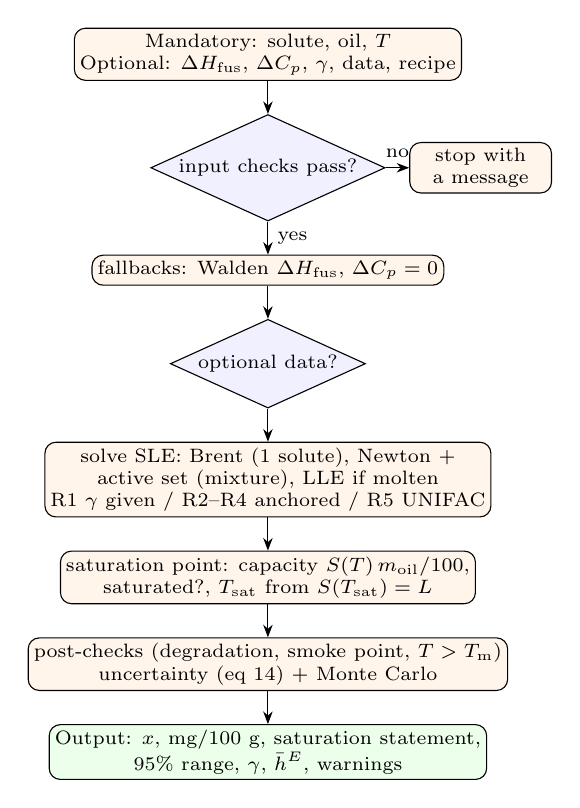
\begin{tikzpicture}[node distance=4.2mm, every node/.style={font=\scriptsize, align=center},
 box/.style={draw, rounded corners, fill=orange!8, minimum width=30mm, inner sep=2pt},
 dec/.style={draw, diamond, aspect=2.2, fill=blue!6, inner sep=1pt},
 arr/.style={-{Stealth[length=1.6mm]}}]
\node[box] (in) {Mandatory: solute, oil, $T$\\ Optional: $\Delta H_\mathrm{fus}$, $\Delta C_p$, $\gamma$, data, recipe};
\node[dec, below=of in] (chk) {input checks pass?};
\node[box, right=3mm of chk, minimum width=18mm] (stop) {stop with\\a message};
\node[box, below=of chk] (fb) {fallbacks: Walden $\Delta H_\mathrm{fus}$, $\Delta C_p=0$};
\node[dec, below=of fb] (route) {optional data?};
\node[box, below=of route] (solve) {solve SLE: Brent (1 solute), Newton +\\active set (mixture), LLE if molten\\R1 $\gamma$ given / R2--R4 anchored / R5 UNIFAC};
\node[box, below=of solve] (sat) {saturation point: capacity $S(T)\,m_\mathrm{oil}/100$,\\saturated?, $T_\mathrm{sat}$ from $S(T_\mathrm{sat})=L$};
\node[box, below=of sat] (post) {post-checks (degradation, smoke point, $T>T_\mathrm{m}$)\\uncertainty (eq 14) + Monte Carlo};
\node[box, below=of post, fill=green!8] (out) {Output: $x$, mg/100 g, saturation statement,\\95\% range, $\gamma$, $\bar h^E$, warnings};
\draw[arr] (in)--(chk); \draw[arr] (chk)--node[above]{no}(stop); \draw[arr] (chk)--node[right]{yes}(fb);
\draw[arr] (fb)--(route); \draw[arr] (route)--(solve); \draw[arr] (solve)--(sat); \draw[arr] (sat)--(post); \draw[arr] (post)--(out);
\end{tikzpicture}
\caption{Workflow of the tool. The decision on optional data selects routes R1--R5; the saturation-point step turns the solubility into the capacity of the pan, a saturated/not-saturated verdict and the saturation temperature.}
\label{fig:workflow}
\end{figure}

\section{Computational Details}
The tool is a Python package (NumPy, SciPy, Matplotlib)\cite{numpy2020,scipy2020,matplotlib2007} organised along the five group roles: data, single-solute solver, mixture solver, validation and checks, and analysis (Figure~\ref{fig:workflow}). \textit{Single solute.} $\ln a_s=\ln x+\ln\gamma_s$ is first evaluated on a 450-point grid spanning $10^{-12}<x<1-10^{-9}$, which detects non-monotonic behaviour and brackets the root on the oil-rich side. Brent's method\cite{brent1973} in $u=\ln x$ then converges to $|F|<10^{-13}$ in five iterations (Figure~\ref{fig:conv}a). Liquid--liquid equilibria are initialised from the lower convex hull of $\Delta G_\mathrm{mix}/RT$ and refined by a Powell hybrid solver in $\ln x'$ and $\ln(1-x'')$. \textit{Mixtures.} Newton--Raphson on eq~\ref{eq:mix} uses a central-difference Jacobian, a trust limit of 2 on $|\Delta u|$ and step halving until $\lVert F\rVert$ decreases; started from the single-solute solutions, three iterations reach $\max|F_i|<10^{-12}$ (Figure~\ref{fig:conv}b). \textit{Saturation point.} The module \texttt{saturation.py} implements the subsection ``Determining the saturation point; command-line access is \texttt{python -m flavorsol saturation} (one compound) and \texttt{python -m flavorsol mixsat} (mixtures).

\textit{Website.} A single-file web application (React, Recharts) lets the user choose compound, oil, temperature, oil mass and amounts added, and shows the saturation statement, the capacity, the undissolved amount and the saturation temperature on the solubility curve; a Mixtures tab does the same for recipes with several compounds, and a Methodology tab documents the method. It runs without a server: single-compound values are the Python solubility curves at 1~K steps, and the mixture equations are solved in the browser by a line-by-line port of the UNIFAC and Newton--Raphson code using the same parameter file. An automated test compares the port with Python on 48 mixture cases (largest relative difference $1.5\times10^{-13}$) and 30 saturation cases (saturation temperatures within 0.001~K).

\textit{Verification.} 37 automated tests check the DDBST reference solution; $\gamma\to1$ for a pure component; the Gibbs--Duhem relation; atom counts of every group assignment; recovery of the ideal solubility when the solvent is chemically identical to the solute; the equilibrium residual; equal activities in both liquid phases; agreement between mixture and single-solute solvers; mass balances; unit conversions; route selection; the Walden fallback; the boundary checks; eq~\ref{eq:dlnx} against finite differences; delta-method versus Monte Carlo intervals; and, for the saturation module, the mass balance, the saturated/not-saturated verdicts, the monotonic rise of $S(T)$ for all six compound--oil pairs and that $T_\mathrm{sat}$ is the root of eq~\ref{eq:Tsat}. The complete study runs with \texttt{python run\_all.py} in about ten minutes and also writes every input and output file of the Data folder.

\section{Results and Discussion}

\subsection{Verification and validation}
\textit{UNIFAC implementation.} For n-hexane/2-butanone at 333.15~K and $x_1=0.5$ the code returns $\gamma=(1.427603, 1.364655)$, identical to the DDBST reference solution within $6\times10^{-11}$.

\textit{Thermodynamic consistency.} For every compound--oil pair and every temperature the predicted activity coefficient at saturation is above one (minimum 1.003 for piperine near its melting point, 5.9 for vanillin and 21.9 for curcumin), so every predicted $x_s$ lies below the ideal-solution limit, as the second law requires for a solute that mixes endothermically. $S(T)$ increases monotonically from 25 to 200~$^\circ$C in all six cases, $\ln\gamma\to0$ in the pure-solute limit to $10^{-15}$, and the ideal solubility reaches one at $T_\mathrm{m}$, beyond which the limit becomes full miscibility (piperine) or a liquid--liquid split (vanillin, curcumin) that joins the SLE branch continuously.

\textit{Vanillin analogues in pure solvents.} Ethyl vanillin\cite{wu2017} and vanillyl alcohol\cite{guo2017} share vanillin's guaiacol core. Their solubilities in alcohols, acetone and acetate esters were retrieved from the NIST ThermoML archive\cite{thermoml} (78 points, 273--343~K). Table~\ref{tab:solv} and Figure~\ref{fig:valid}a compare predictions with these data. In the aprotic solvents, whose ester and ketone groups resemble the triglyceride's ester linkages, UNIFAC gives an average absolute relative deviation (AARD) of 46\%, against 65\% for the ideal solution. The ideal model fails as the solvent becomes less polar, reaching 253\% for vanillyl alcohol in butyl acetate (UNIFAC: 38\%). In short alcohols, UNIFAC over-predicts the attraction between phenolic OH and alcohol OH groups (AARD 105\% versus 54\%), a known weakness that does not apply to anhydrous oils. For vanillin's octanol--water partition coefficient, UNIFAC gives $\log K_\mathrm{ow}=1.35$ against 1.23 measured.\cite{oecd_vanillin}

\begin{table}
\caption{Validation in Pure Solvents (AARD, \%)}
\label{tab:solv}
\small
\resizebox{\columnwidth}{!}{\begin{tabular}{llcccc}
\toprule
solute & solvent & $n$ & $T$ (K) & UNIFAC & ideal\\
\midrule
EV & ethanol & 10 & 273--318 & 88 & 34 \\
EV & 1-propanol & 10 & 273--318 & 110 & 63 \\
EV & 2-propanol & 10 & 273--318 & 157 & 95 \\
EV & acetone & 10 & 273--318 & 5 & 32 \\
EV & methyl acetate & 10 & 273--318 & 47 & 9 \\
EV & ethyl acetate & 10 & 273--318 & 39 & 7 \\
VA & ethanol & 6 & 293--343 & 40 & 5 \\
VA & ethyl acetate & 6 & 293--343 & 130 & 121 \\
VA & butyl acetate & 6 & 293--343 & 38 & 253 \\
\bottomrule
\end{tabular}}

\footnotesize EV, ethyl vanillin;\cite{wu2017} VA, vanillyl alcohol.\cite{guo2017}
\end{table}

\begin{table}
\caption{Solubility in Oils (mg per mL oil)}
\label{tab:oils}
\small
\resizebox{\columnwidth}{!}{\begin{tabular}{llcccc}
\toprule
solute & oil & $t$/$^\circ$C & publ.$^a$ & UNIFAC & ideal\\
\midrule
piperine & MCT & 37 & 3.93 & 6.6 & 16 \\
curcumin & MCT & 25 & 0.25 & 0.42 & 3.9 \\
curcumin & coconut & 25 & 0.1 & 0.081 & 2.9 \\
curcumin & olive & 25 & 0.08 & 0.025 & 2.1 \\
curcumin & corn & 25 & 0.07 & 0.03 & 2.2 \\
curcumin & corn & 100 & 3.5 & 0.88 & 50 \\
curcumin & MCT & 100 & 6$^{c}$ & 6.5 & 88 \\
curcumin & MCT & 25 & 12.4$^{d}$ & 0.42 & 3.9 \\
curcumin & sunflower & 25 & 5.4$^{d}$ & 0.03 & 2.2 \\
curcumin & corn & 25 & 6.2$^{d}$ & 0.03 & 2.2 \\
\bottomrule
\end{tabular}}

\footnotesize $^a$References \citenum{araiza2018,kusumorini2022}. $^c$Lower bound. $^d$Above the ideal-solution limit; excluded from statistics.
\end{table}

\textit{Edible oils.} Table~\ref{tab:oils} and Figure~\ref{fig:valid}b compare predictions with published solubilities in oils. For the six equilibrium values (curcumin at 25~$^\circ$C in MCT, coconut, olive and corn oils, curcumin at 100~$^\circ$C in corn oil, and piperine at 37~$^\circ$C in MCT) the mean absolute deviation is 0.33 in $\log_{10}$ (a factor of 2.2) and the worst case is a factor of 4.0. The ideal solution over-predicts by a factor of about 20 (AARD 1900\%). UNIFAC also reproduces the measured ranking of curcumin solubility, MCT $>$ coconut $>$ olive $\approx$ corn, which follows from shorter acyl chains carrying more ester groups per CH$_2$. A second cluster of curcumin reports (5--12~mg/mL at ambient temperature) disagrees with the first by up to two orders of magnitude. With $\gamma\ge1$, which is expected for a polar hydrogen-bond donor in a triglyceride, the solubility cannot exceed the ideal value: 2.2~mg/mL in sunflower or corn oil and 3.9~mg/mL in MCT. Values above this limit imply $\gamma<1$, or that the solid was not the stable crystal (supersaturation after heating, amorphous or less stable forms,\cite{liu2015} impure curcuminoid mixtures), or that undissolved colloids were counted.

\begin{figure*}
\centering
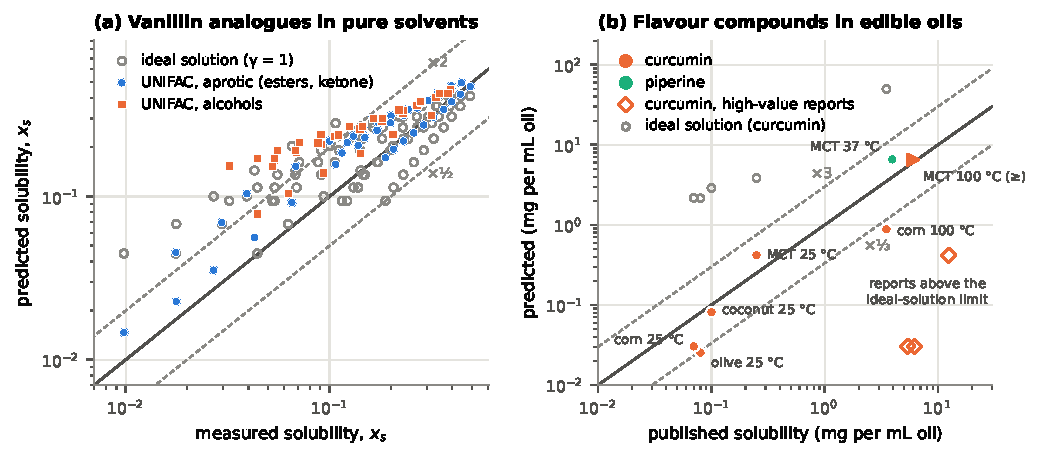
\includegraphics[width=0.95\textwidth]{fig2_validation.pdf}
\caption{Validation. (a) Analogue solutes in pure solvents; dashed lines mark a factor of 2. (b) Published solubilities in edible oils. Filled symbols are equilibrium values, the triangle is a lower bound, open diamonds are reports above the ideal-solution limit; dashed lines mark a factor of 3.}
\label{fig:valid}
\end{figure*}

\textit{Data-anchored routes.} Leave-out tests on the analogue data quantify how much one measurement helps (Figure~\ref{fig:extrap}b). Predicting other temperatures in the same solvent from the lowest-temperature point (69 predictions) lowers the AARD from 65\% (pure UNIFAC) to 28\% with anchored UNIFAC, 24\% with constant $\gamma$, and 20\% with the regular-solution assumption. Transferring a 25~$^\circ$C point to every other solvent (336 predictions, route R3) lowers the AARD from 74\% to 48\%. In oil, anchoring curcumin in corn oil at 25~$^\circ$C (0.07~mg/mL) and extrapolating 75~K raises the 100~$^\circ$C prediction from 96 to 225~mg/100~g (regular solution: 312), against 326--435~mg/100~g measured; the anchored 95\% range (92--553) contains the measurement (Figure~\ref{fig:extrap}a).

\begin{figure*}
\centering
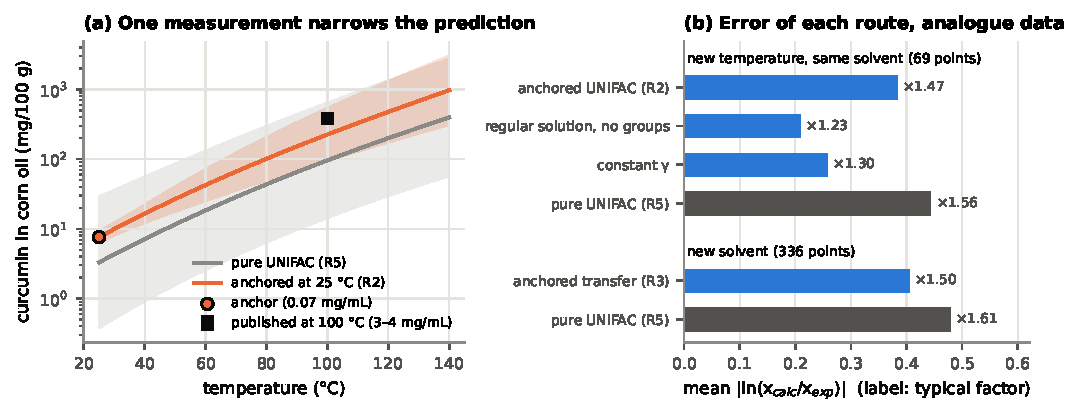
\includegraphics[width=0.95\textwidth]{fig8_extrapolation_uncertainty.pdf}
\caption{(a) Curcumin in corn oil: pure prediction and prediction anchored on one 25~$^\circ$C measurement, with 95\% ranges. (b) Mean $|\ln(x_\mathrm{calc}/x_\mathrm{exp})|$ of each route in leave-out tests on the analogue data.}
\label{fig:extrap}
\end{figure*}

\subsection{Solubility from room temperature to frying}
Table~\ref{tab:pred} and Figure~\ref{fig:solT} give the predicted solubilities. Curcumin is the least soluble compound: 3.3~mg/100~g in sunflower oil at 25~$^\circ$C, about 70 times below its ideal solubility. Its solubility rises 30-fold to 97~mg/100~g at 100~$^\circ$C and 430-fold to 1430~mg/100~g at 180~$^\circ$C, because its fusion enthalpy is large and its melting point high. Piperine is nearly ideal ($\gamma^\infty=2$--3). It dissolves at 0.2--0.25~g/100~g at room temperature, 8.5--8.7~g/100~g at 100~$^\circ$C, and becomes fully miscible above its melting point (133~$^\circ$C). Vanillin reaches 0.4--0.7~g/100~g at 25~$^\circ$C. Above its 82~$^\circ$C melting point molten vanillin and oil are only partly miscible: the oil-rich phase holds 3--7~g/100~g. Coconut oil dissolves 1.7--2.7 times more curcumin and 1.4--1.8 times more vanillin than sunflower oil at the same temperature; piperine is slightly more soluble in sunflower oil up to 100~$^\circ$C.

\begin{table}
\caption{Predicted Solubility (mg per 100 g oil)$^a$}
\label{tab:pred}
\scriptsize
\resizebox{\columnwidth}{!}{\begin{tabular}{llccccc}
\toprule
compound & oil & 25~$^\circ$C & 60~$^\circ$C & 100~$^\circ$C & 140~$^\circ$C & 180~$^\circ$C\\
\midrule
vanillin & sunflower & 420 & 1390 & 3200$^{b}$ & 3950$^{b}$ & 4840$^{b}$ \\
vanillin & coconut & 739 & 2280 & 5050$^{b}$ & 5790$^{b}$ & 6740$^{b}$ \\
curcumin & sunflower & 3.32 & 18.5 & 97 & 399 & 1430 \\
curcumin & coconut & 8.81 & 40.9 & 186 & 700 & 2450 \\
piperine & sunflower & 245 & 1410 & 8700 & miscible & miscible \\
piperine & coconut & 218 & 1310 & 8520 & miscible & miscible \\
\bottomrule
\end{tabular}}

\footnotesize $^a$Pure UNIFAC (route R5); typical uncertainty a factor of 2--3. $^b$Above $T_\mathrm{m}$: molten vanillin forms a second liquid phase; the value is the oil-rich-phase composition.
\end{table}

\begin{figure*}
\centering
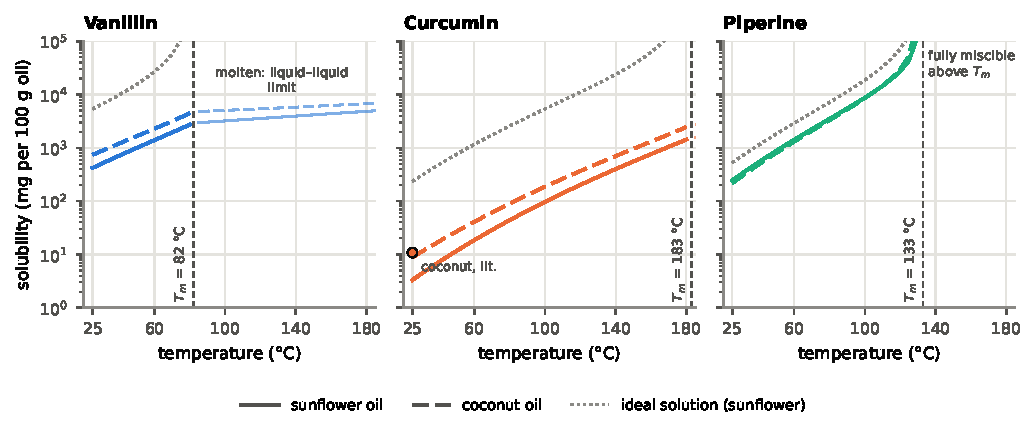
\includegraphics[width=0.95\textwidth]{fig3_solubility_vs_T.pdf}
\caption{Predicted solubility versus temperature. The vertical dashed line is the melting point; the dotted line is the ideal solution in sunflower oil; the circle is a published value for curcumin in coconut oil.}
\label{fig:solT}
\end{figure*}

\subsection{Origin of the non-ideality}
Table~\ref{tab:thermo} and Figure~\ref{fig:gamma} split $\ln\gamma^\infty$ into its UNIFAC parts. The residual term dominates for every pair. It is largest for curcumin (4.6 in sunflower oil), whose two phenolic OH, two methoxy and two carbonyl groups interact unfavourably with CH$_2$-rich chains. The combinatorial term is negative because the oil molecules are much larger than the solutes, and more negative in sunflower oil (C18 chains) than in coconut oil (mostly C12). Coconut oil's advantage therefore comes from its higher density of ester groups, which lowers the residual term from 4.55 to 3.65 for curcumin. The apparent enthalpies of dissolution from eq~\ref{eq:dlnx} (25--60~$^\circ$C) are 25--42~kJ\,mol$^{-1}$, within 5~kJ\,mol$^{-1}$ of the fusion enthalpies, so the temperature dependence of solubility, and therefore the saturation temperature of a recipe, is set mainly by melting.

\begin{table}
\caption{Activity Coefficients at 25~$^\circ$C, Apparent Dissolution Enthalpy (25--60~$^\circ$C) and Onset of a Second Liquid Phase}
\label{tab:thermo}
\scriptsize
\resizebox{\columnwidth}{!}{\begin{tabular}{llccccc}
\toprule
 & oil & $\ln\gamma^C$ & $\ln\gamma^R$ & $\gamma^\infty$ & $\Delta H_\mathrm{sol}$ (kJ/mol) & $t_\mathrm{LL}$ ($^\circ$C)\\
\midrule
vanillin & sunflower & -1.09 & 3.42 & 10.2 & 27.0 & 82 \\
vanillin & coconut & -0.84 & 2.90 & 7.9 & 25.1 & 82 \\
curcumin & sunflower & -0.30 & 4.55 & 70.4 & 40.6 & 183 \\
curcumin & coconut & -0.09 & 3.65 & 35.2 & 36.2 & 183 \\
piperine & sunflower & -0.43 & 1.19 & 2.1 & 40.5 & -- \\
piperine & coconut & -0.20 & 1.37 & 3.2 & 41.7 & -- \\
\bottomrule
\end{tabular}}
\end{table}

\begin{figure*}
\centering
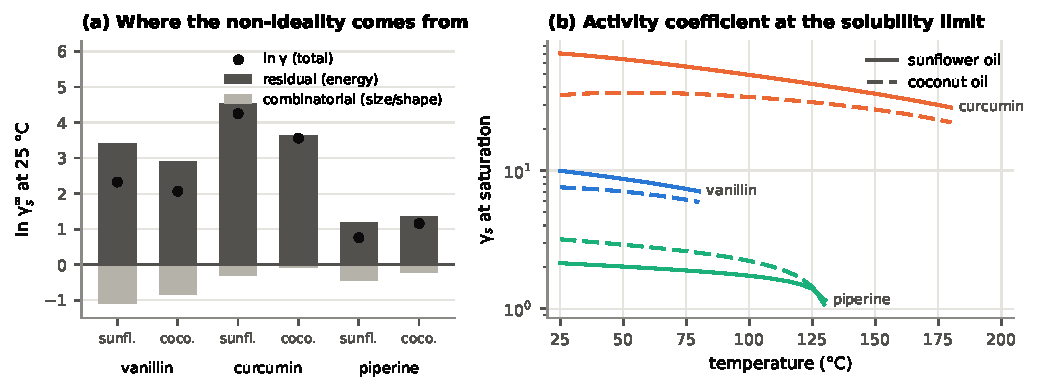
\includegraphics[width=0.95\textwidth]{fig4_activity_coefficients.pdf}
\caption{(a) Combinatorial and residual parts of $\ln\gamma^\infty$ at 25~$^\circ$C. (b) Activity coefficient at the solubility limit versus temperature.}
\label{fig:gamma}
\end{figure*}

\subsection{Saturation point: when no more compound can mix in}
Table~\ref{tab:sat} applies the subsection ``Determining the saturation point to one tadka: 15~g oil with 47~mg curcumin (1.5~g turmeric at 3.14\%\cite{tayyem2006}), 50~mg piperine (1~g black pepper at about 5\%\cite{gorgani2017}) and 15~mg vanillin (0.1\% flavouring level). Each compound is first treated alone. Curcumin is saturated at every ordinary cooking temperature: at 60~$^\circ$C coconut oil can hold only 6.14~mg, so saturation is achieved and more mixing cannot be done, and 40.9~mg (87\%) remains as solid. The loading of 313~mg/100~g meets the solubility curve at $T_\mathrm{sat}=115.2~^\circ$C in coconut oil and 132.8~$^\circ$C in sunflower oil (Figure~\ref{fig:sat}a); only above these temperatures does the oil take up the whole amount. Piperine saturates only near room temperature ($T_\mathrm{sat}=30.7$ and 32.8~$^\circ$C) and vanillin is never saturated at this dose. Figure~\ref{fig:sat}b generalises the result as the saturation temperature versus amount added: at a given loading, curcumin needs 50--80~K more than piperine, and coconut oil lowers the temperature needed for curcumin by about 15--20~K compared with sunflower oil.

\begin{table}
\caption{Saturation Point of a Tadka Recipe in 15~g Oil, Each Compound Alone}
\label{tab:sat}
\scriptsize
\resizebox{\columnwidth}{!}{\begin{tabular}{llcccc}
\toprule
compound (added) & oil & $C$ at 25 / 60 / 100~$^\circ$C (mg) & saturated at 60~$^\circ$C? & $T_\mathrm{sat}$ ($^\circ$C)\\
\midrule
curcumin (47 mg) & sunflower & 0.50 / 2.78 / 14.5 & yes, 44.2 mg left & 132.8\\
curcumin (47 mg) & coconut & 1.32 / 6.14 / 27.9 & yes, 40.9 mg left & 115.2\\
piperine (50 mg) & sunflower & 36.7 / 212 / 1306 & no & 30.7\\
piperine (50 mg) & coconut & 32.7 / 196 / 1278 & no & 32.8\\
vanillin (15 mg) & sunflower & 63.0 / 209 / 480 & no & $<$25\\
vanillin (15 mg) & coconut & 111 / 342 / 757 & no & $<$25\\
\bottomrule
\end{tabular}}
\end{table}

\begin{figure*}
\centering
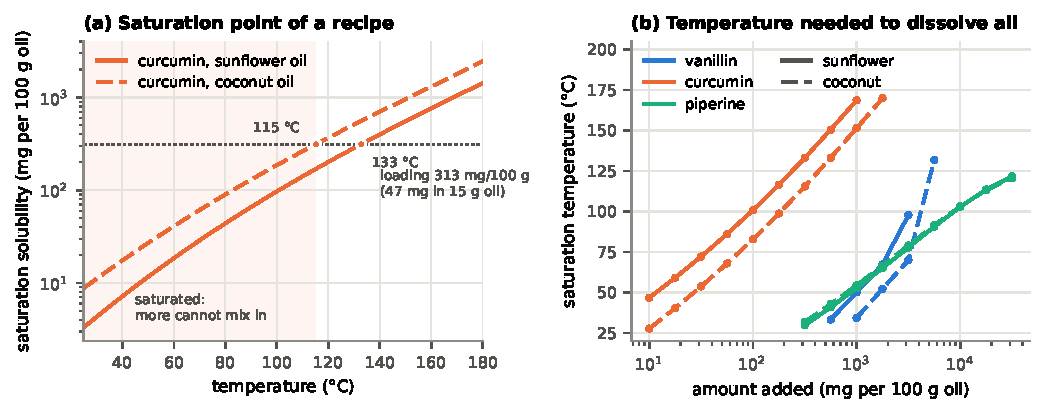
\includegraphics[width=0.95\textwidth]{fig9_saturation_point.pdf}
\caption{(a) Saturation point of the tadka curcumin loading: the solubility curve meets the loading line at the saturation temperature; in the shaded region (coconut oil) the oil is saturated and more curcumin cannot mix in. (b) Saturation temperature versus amount added for all compounds and both oils.}
\label{fig:sat}
\end{figure*}

\textit{Mixtures.} When the three compounds are added together the saturation statements are produced by the mixture solver. At 60~$^\circ$C in coconut oil the tool reports: ``saturation is achieved for curcumin: more mixing cannot be done for this compound'', with 6.39~mg curcumin dissolved (40.6~mg left), while vanillin and piperine dissolve completely and could take about 335 and 148~mg more. In sunflower oil at 60~$^\circ$C curcumin saturates at 2.90~mg. The whole recipe dissolves at 114.1~$^\circ$C in coconut oil and 131.6~$^\circ$C in sunflower oil, about 1~K below the single-compound values, because dissolved vanillin and piperine make the oil slightly more polar. At 25~$^\circ$C both curcumin and piperine are saturated. For a deliberately high loading (1~g vanillin, 0.5~g curcumin, 2~g piperine in 15~g sunflower oil at 140~$^\circ$C) vanillin and curcumin are saturated, the excess vanillin separating as a second liquid layer and the excess curcumin remaining solid, while molten piperine mixes in all proportions. All 24 mixture scenarios and 60 single-compound scenarios are tabulated, with their statements, in the Data folder.

\subsection{Flavour in the pan: mixtures and recipes}
With the illustrative loadings (314, 333 and 100~mg per 100~g oil for curcumin, piperine and vanillin) the mass-limited mixture solver gives the share of each compound that can enter the oil (Figure~\ref{fig:recipe}a). Vanillin always dissolves completely. Piperine dissolves completely above about 35~$^\circ$C. Curcumin is solubility-limited over most of the cooking range: at 25, 60 and 100~$^\circ$C only 1.1, 6.2 and 32\% dissolves in sunflower oil (2.9, 13.6 and 62\% in coconut oil). Thermodynamics thus supports the culinary practice of adding turmeric to hot oil. Relative to sensory thresholds, dissolved vanillin is about $5\times10^4$ times above its odour threshold in water\cite{plotto2004} and piperine about $5\times10^3$ times above its detection threshold,\cite{spence2024} so for these two compounds release from the spice and evaporation govern perceived intensity, not solubility.

Table~\ref{tab:mix} gives every pair and the three-way mixture with all compounds present as excess solid. Vanillin raises curcumin's solubility (up to $\times1.81$ at 75~$^\circ$C in coconut oil), vanillin and piperine help each other slightly, and curcumin and piperine barely interact, partly because the phenol--amide interaction parameter is unpublished and set to zero. When all three are present as excess solids (Figure~\ref{fig:recipe}b) each dissolves slightly more than it would alone, most strongly curcumin ($\times1.12$--2.4 between 25 and 75~$^\circ$C). The predicted competition between compounds is therefore cooperative (co-solvency); at recipe loadings the effect is only about 4\%. Each compound is assumed to crystallise as its own pure solid; co-amorphous curcumin--piperine solids are known, so the residual solid of mixture experiments should be checked by DSC.

\begin{table*}
\caption{Solubility of Each Compound in a Mixture Divided by Its Solubility Alone (All Compounds in Excess)$^a$}
\label{tab:mix}
\small
\begin{tabular}{llcccccc}
\toprule
 & & \multicolumn{3}{c}{sunflower oil} & \multicolumn{3}{c}{coconut oil}\\
mixture & compound & 25~$^\circ$C & 60~$^\circ$C & 75~$^\circ$C & 25~$^\circ$C & 60~$^\circ$C & 75~$^\circ$C\\
\midrule
V + C & vanillin & 1.00 & 1.00 & 1.01 & 1.00 & 1.00 & 1.01 \\
V + C & curcumin & 1.10 & 1.31 & 1.53 & 1.15 & 1.46 & 1.81 \\
V + P & vanillin & 1.01 & 1.09 & 1.20 & 1.01 & 1.08 & 1.21 \\
V + P & piperine & 1.04 & 1.14 & 1.26 & 1.07 & 1.23 & 1.43 \\
C + P & curcumin & 1.02 & 1.10 & 1.20 & 1.01 & 1.09 & 1.18 \\
C + P & piperine & 1.00 & 1.00 & 1.00 & 1.00 & 1.00 & 1.00 \\
V + C + P & vanillin & 1.01 & 1.09 & 1.21 & 1.01 & 1.09 & 1.23 \\
V + C + P & curcumin & 1.12 & 1.48 & 2.01 & 1.16 & 1.65 & 2.43 \\
V + C + P & piperine & 1.04 & 1.14 & 1.27 & 1.07 & 1.23 & 1.45 \\
\bottomrule
\end{tabular}

\footnotesize $^a$V, vanillin; C, curcumin; P, piperine. Values above 1 mean the other compounds increase the solubility.
\end{table*}

\begin{figure*}
\centering
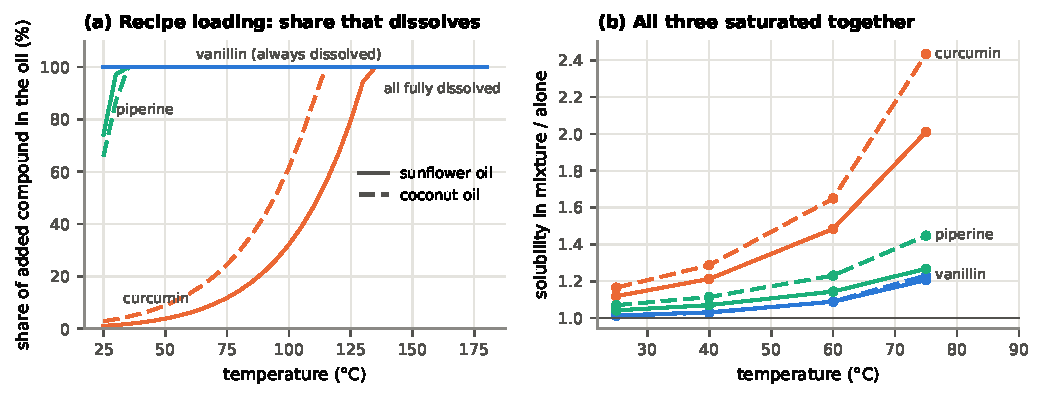
\includegraphics[width=0.95\textwidth]{fig5_recipe_and_mixture.pdf}
\caption{(a) Share of each compound added in the tadka that dissolves in the oil. (b) Solubility of each compound when all three are saturated together, relative to its solubility alone.}
\label{fig:recipe}
\end{figure*}

\subsection{Sensitivity and limitations}
At 60~$^\circ$C in sunflower oil (Figure~\ref{fig:sens}), curcumin is most sensitive to $\Delta C_p$ ($+72\%$ if $\Delta C_p=\Delta S_\mathrm{fus}$), to its group representation ($-63\%$ for the keto--enol form) and to $\Delta H_\mathrm{fus}$ ($+44/-30\%$ for $\mp10\%$). Literature values of curcumin's $\Delta H_\mathrm{fus}$ span roughly 37--49~kJ\,mol$^{-1}$, so a DSC measurement on the group's own sample would sharpen the predictions, and the saturation temperatures, more than any change to the model. Vanillin is most sensitive to the UNIFAC parameters and $T_\mathrm{m}$, piperine to its fusion data. Changing sunflower oil to a high-oleic variety lowers all three solubilities by 11--19\%.

The main limitations are: (i) UNIFAC errors of a factor of 1.5--2.5 for these multifunctional solutes, which the anchored routes reduce; (ii) one pseudo-triglyceride for each oil, which ignores minor components (free fatty acids, mono- and diglycerides, water) that can raise the solubility of polar solutes; (iii) parameters fitted mostly below 150~$^\circ$C, so frying-temperature predictions are extrapolations; (iv) equilibrium only, whereas real cooking also involves release from the spice matrix, degradation and evaporation (flagged, not modelled), so the saturation point is a thermodynamic upper bound on what the oil takes up; and (v) polymorphism and tautomerism of curcumin.

\begin{figure*}
\centering
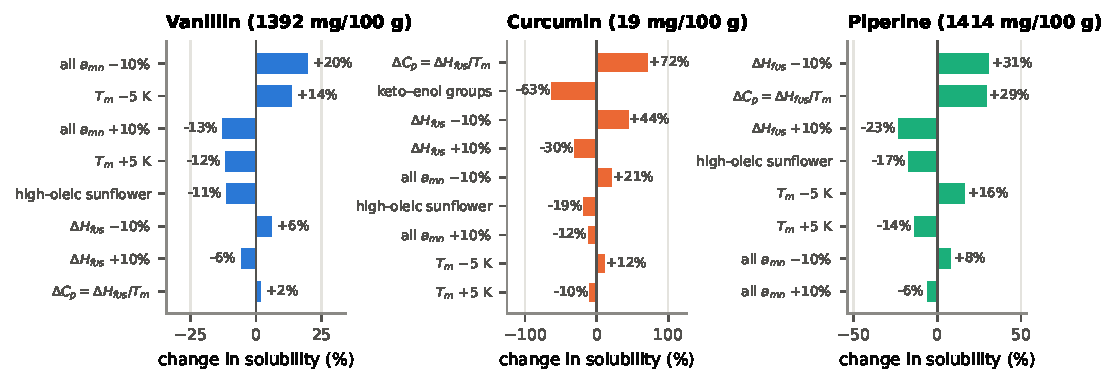
\includegraphics[width=0.95\textwidth]{fig6_sensitivity.pdf}
\caption{Change in predicted solubility at 60~$^\circ$C in sunflower oil for each perturbed input.}
\label{fig:sens}
\end{figure*}

\begin{figure}
\centering
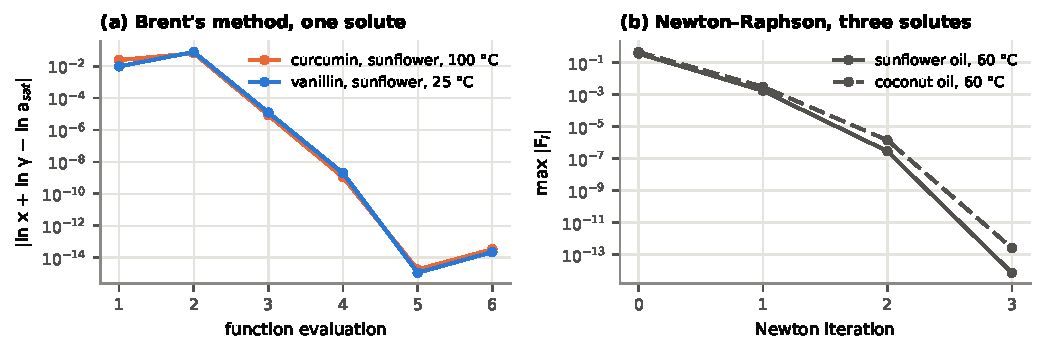
\includegraphics[width=\columnwidth]{fig7_convergence.pdf}
\caption{Convergence of (a) Brent's method and (b) Newton--Raphson for the three-solute mixture at 60~$^\circ$C.}
\label{fig:conv}
\end{figure}

\section{Conclusions}
A tested, modular Python tool and an offline website now predict the solubility of flavour compounds in cooking oils from fusion properties and UNIFAC. The tool handles one or several compounds, mass-limited recipes, melting and liquid--liquid splitting, and for every case states whether saturation is achieved at the chosen temperature, how much cannot be mixed in, and the saturation temperature above which the whole amount dissolves. It adapts to the data the user has, through five routes from pure prediction to anchoring on a single measurement, and reports uncertainty and degradation risks alongside each number. All predictions satisfy the thermodynamic consistency checks ($\gamma\ge1$, $x_s\le x_\mathrm{ideal}$, $S(T)$ rising with $T$, Gibbs--Duhem). Against published data in oils the model is accurate to a factor of about 2, ten times better than the ideal-solution model. Curcumin is the solubility-limited flavour compound: a typical tadka saturates the oil with curcumin below 115~$^\circ$C (coconut) or 133~$^\circ$C (sunflower), whereas piperine and vanillin dissolve completely at culinary doses. The next steps are DSC measurements of the group's own samples, solubility measurements in the two oils at 25--120~$^\circ$C to anchor and test the model and its saturation temperatures, and screening further spice molecules from FlavorDB2 and SpiceRx.

\section*{Data and Code Availability}
The Python package, website, input files, output data for every scenario, and scripts that regenerate every table and figure (\texttt{run\_all.py}) are provided with this manuscript in the folders Codes and Data, and at \url{https://github.com/Janil-ship-it/spice-oil-solubility}. The website is the single file \path{Codes/website/dist/index.html}, which opens in any browser without installation.

\begin{acknowledgement}
We thank Prof.\ Kaustubh Rane and the teaching assistant Mayank Makwana for guidance and feedback during the project reviews, including the suggestion to use FlavorDB and SpiceRx.
\end{acknowledgement}

\section*{Author Contributions}
All authors (Rohan Jaybhave, Janil Jain, Preet Patel, Saksham Malav and Manish Kumawat) contributed to the property and oil databases, the single-solute and mixture solvers, validation and boundary checks, the saturation-point analysis, the website, and the analysis and figures, and all authors wrote and reviewed the manuscript.

\begin{thebibliography}{99}
\bibitem{prausnitz1999} Prausnitz, J.~M.; Lichtenthaler, R.~N.; Gomes de Azevedo, E. \textit{Molecular Thermodynamics of Fluid-Phase Equilibria}, 3rd ed.; Prentice Hall: Upper Saddle River, NJ, 1999.
\bibitem{smith2018} Smith, J.~M.; Van Ness, H.~C.; Abbott, M.~M.; Swihart, M.~T. \textit{Introduction to Chemical Engineering Thermodynamics}, 8th ed.; McGraw-Hill: New York, 2018.
\bibitem{fredenslund1975} Fredenslund, A.; Jones, R.~L.; Prausnitz, J.~M. Group-Contribution Estimation of Activity Coefficients in Nonideal Liquid Mixtures. \textit{AIChE J.} \textbf{1975}, \textit{21}, 1086--1099.
\bibitem{hansen1991} Hansen, H.~K.; Rasmussen, P.; Fredenslund, A.; Schiller, M.; Gmehling, J. Vapor-Liquid Equilibria by UNIFAC Group Contribution. 5. Revision and Extension. \textit{Ind. Eng. Chem. Res.} \textbf{1991}, \textit{30}, 2352--2355.
\bibitem{gracin2002} Gracin, S.; Brinck, T.; Rasmuson, \AA.~C. Prediction of Solubility of Solid Organic Compounds in Solvents by UNIFAC. \textit{Ind. Eng. Chem. Res.} \textbf{2002}, \textit{41}, 5114--5124.
\bibitem{araiza2018} Araiza-Calahorra, A.; Akhtar, M.; Sarkar, A. Recent Advances in Emulsion-Based Delivery Approaches for Curcumin: From Encapsulation to Bioaccessibility. \textit{Trends Food Sci. Technol.} \textbf{2018}, \textit{71}, 155--169.
\bibitem{zou2016} Zou, L.; Zheng, B.; Zhang, R.; et al. Influence of Lipid Phase Composition of Excipient Emulsions on Curcumin Solubility, Stability, and Bioaccessibility. \textit{Food Biophys.} \textbf{2016}, \textit{11}, 213--225.
\bibitem{kusumorini2022} Kusumorini, N.; Nugroho, A.~K.; Pramono, S.; Martien, R. Spray-Dried Self-Nanoemulsifying Drug Delivery Systems as Carriers for the Oral Delivery of Piperine: Characterization and in Vitro Evaluation. \textit{J. Appl. Pharm. Sci.} \textbf{2022}, \textit{12}, 43--57.
\bibitem{wu2017} Wu, H.; Wang, J.; Zhou, Y.; Guo, N.; Liu, Q.; Zong, S.; Bao, Y.; Hao, H. Solid-Liquid Phase Equilibrium and Dissolution Properties of Ethyl Vanillin in Pure Solvents. \textit{J. Chem. Thermodyn.} \textbf{2017}, \textit{105}, 345--351.
\bibitem{guo2017} Guo, Y.; Hao, Y.; Zhou, Y.; Han, Z.; Xie, C.; Su, W.; Hao, H. Solubility and Thermodynamic Properties of Vanillyl Alcohol in Some Pure Solvents. \textit{J. Chem. Thermodyn.} \textbf{2017}, \textit{106}, 276--284.
\bibitem{garg2018} Garg, N.; et al. FlavorDB: A Database of Flavor Molecules. \textit{Nucleic Acids Res.} \textbf{2018}, \textit{46}, D1210--D1216.
\bibitem{rakhi2018} Rakhi, N.~K.; Tuwani, R.; Mukherjee, J.; Bagler, G. Data-Driven Analysis of Biomedical Literature Suggests Broad-Spectrum Benefits of Culinary Herbs and Spices. \textit{PLoS One} \textbf{2018}, \textit{13}, e0198030.
\bibitem{nist_vanillin} National Institute of Standards and Technology. Vanillin, NIST Chemistry WebBook, SRD 69: Phase Change Data. \url{https://webbook.nist.gov/cgi/cbook.cgi?ID=C121335&Mask=4} (accessed Nov 8, 2026).
\bibitem{pubchem_curcumin} National Center for Biotechnology Information. PubChem Compound Summary for CID 969516, Curcumin. \url{https://pubchem.ncbi.nlm.nih.gov/compound/969516} (accessed Nov 8, 2026).
\bibitem{fitriani2023} Fitriani, L.; Simbolon, C.~A.; Zaini, E. Preparation and Characterization of Multicomponent Crystal Piperine-Caffeine. \textit{J. Sains Farm. Klin.} \textbf{2023}, \textit{10}, 353--358.
\bibitem{temprado2008} Temprado, M.; Roux, M.~V.; Chickos, J.~S. Some Thermophysical Properties of Several Solid Aldehydes. \textit{J. Therm. Anal. Calorim.} \textbf{2008}, \textit{94}, 257--262.
\bibitem{ranjbar2024} Ranjbar, M.; Vashishtha, M.; Gadipelli, S.; Ramisetty, K.; Walker, G.; Brett, D.~J.~L.; Vasanth Kumar, K. Pseudo Second Order Kinetic Expression to Predict the Kinetics of the Anomalous Crystal Growth of Curcumin in Impure Solution. \textit{CrystEngComm} \textbf{2024}, \textit{26}, 1077--1089.
\bibitem{ddbst} DDBST GmbH. Parameters of the Original UNIFAC Model (Published Parameters). \url{https://www.ddbst.com/published-parameters-unifac.html} (accessed Nov 8, 2026).
\bibitem{manolova2014} Manolova, Y.; Deneva, V.; Antonov, L.; Drakalska, E.; Momekova, D.; Lambov, N. The Effect of the Water on the Curcumin Tautomerism: A Quantitative Approach. \textit{Spectrochim. Acta, Part A} \textbf{2014}, \textit{132}, 815--820.
\bibitem{codex} FAO/WHO Codex Alimentarius Commission. \textit{Standard for Named Vegetable Oils}, CXS 210-1999; FAO/WHO: Rome, as amended.
\bibitem{hansen2007} Hansen, C.~M. \textit{Hansen Solubility Parameters: A User's Handbook}, 2nd ed.; CRC Press: Boca Raton, FL, 2007.
\bibitem{walden1908} Walden, P. \"Uber die Schmelzw\"arme, spezifische Koh\"asion und Molekulargr\"o\ss e bei der Schmelztemperatur. \textit{Z. Elektrochem.} \textbf{1908}, \textit{14}, 713--724.
\bibitem{goel2024} Goel, M.; et al. FlavorDB2: An Updated Database of Flavor Molecules. \textit{J. Food Sci.} \textbf{2024}, \textit{89}, 7076--7082.
\bibitem{rakhi2018spicerx} Rakhi, N.~K.; Tuwani, R.; Garg, N.; Mukherjee, J.; Bagler, G. SpiceRx: An Integrated Resource for the Health Impacts of Culinary Spices and Herbs. \textit{bioRxiv} \textbf{2018}, 273599.
\bibitem{smokepoint} Wikipedia contributors. Smoke Point, table of smoke points. \url{https://en.wikipedia.org/wiki/Smoke_point} (accessed Nov 8, 2026).
\bibitem{siddiqui2015} Siddiqui, N.~A. Evaluation of Thermo Sensitivity of Curcumin and Quantification of Ferulic Acid and Vanillin as Degradation Products by a Validated HPTLC Method. \textit{Pak. J. Pharm. Sci.} \textbf{2015}, \textit{28}, 299--305.
\bibitem{doctor2020} Doctor, N.; Parker, G.; Vang, K.; Smith, M.; Kayan, B.; Yang, Y. Stability and Extraction of Vanillin and Coumarin under Subcritical Water Conditions. \textit{Molecules} \textbf{2020}, \textit{25}, 1061.
\bibitem{kotte2014} Kotte, S.~C.~B.; Dubey, P.~K.; Murali, P.~M. Identification and Characterization of Stressed Degradation Products of Piperine and Profiling with Black Pepper (\textit{Piper nigrum} L.) Extraction by Using LC/Q-TOF-Dual ESI-MS Experiments. \textit{Anal. Methods} \textbf{2014}, DOI: 10.1039/C4AY01088D.
\bibitem{jcgm2008} JCGM. \textit{Evaluation of Measurement Data: Guide to the Expression of Uncertainty in Measurement} (JCGM 100:2008); Joint Committee for Guides in Metrology, 2008.
\bibitem{numpy2020} Harris, C.~R.; et al. Array Programming with NumPy. \textit{Nature} \textbf{2020}, \textit{585}, 357--362.
\bibitem{scipy2020} Virtanen, P.; et al. SciPy 1.0: Fundamental Algorithms for Scientific Computing in Python. \textit{Nat. Methods} \textbf{2020}, \textit{17}, 261--272.
\bibitem{matplotlib2007} Hunter, J.~D. Matplotlib: A 2D Graphics Environment. \textit{Comput. Sci. Eng.} \textbf{2007}, \textit{9}, 90--95.
\bibitem{brent1973} Brent, R.~P. \textit{Algorithms for Minimization without Derivatives}; Prentice-Hall: Englewood Cliffs, NJ, 1973.
\bibitem{thermoml} NIST Thermodynamics Research Center. ThermoML Archive. \url{https://trc.nist.gov/ThermoML/}, data sets 10.1016/j.jct.2016.10.029 and 10.1016/j.jct.2016.11.030 (accessed Nov 8, 2026).
\bibitem{oecd_vanillin} OECD. \textit{SIDS Initial Assessment Report: Vanillin (CAS No. 121-33-5)}; UNEP Publications, OECD High Production Volume Chemicals Programme.
\bibitem{liu2015} Liu, J.; Sv\"ard, M.; Hippen, P.; Rasmuson, \AA.~C. Solubility and Crystal Nucleation in Organic Solvents of Two Polymorphs of Curcumin. \textit{J. Pharm. Sci.} \textbf{2015}, \textit{104}, 2183--2189.
\bibitem{tayyem2006} Tayyem, R.~F.; Heath, D.~D.; Al-Delaimy, W.~K.; Rock, C.~L. Curcumin Content of Turmeric and Curry Powders. \textit{Nutr. Cancer} \textbf{2006}, \textit{55}, 126--131.
\bibitem{gorgani2017} Gorgani, L.; Mohammadi, M.; Najafpour, G.~D.; Nikzad, M. Piperine, the Bioactive Compound of Black Pepper: From Isolation to Medicinal Formulations. \textit{Compr. Rev. Food Sci. Food Saf.} \textbf{2017}, \textit{16}, 124--140.
\bibitem{plotto2004} Plotto, A.; Margar\'ia, C.~A.; Goodner, K.~L.; Goodrich, R.; Baldwin, E.~A. Odour and Flavour Thresholds for Key Aroma Components in an Orange Juice Matrix: Terpenes and Aldehydes. \textit{Flavour Fragrance J.} \textbf{2004}, \textit{19}, 491--498.
\bibitem{spence2024} Spence, C. The King of Spices: On Pepper's Pungent Pleasure. \textit{Int. J. Gastron. Food Sci.} \textbf{2024}, \textit{35}, 100900.
\end{thebibliography}

\end{document}
